\section{Dữ liệu 1}
Những thông tin vê các giám đốc điều hành các tập đoàn Hoa Kỳ. Bộ dữ liệu gồm 177 quan trắc và 15 biến.

$*$ \textbf{Phương pháp chọn: Stepwise - tiến; tiêu chuẩn chọn: AIC}.

\subsection*{Tìm hiểu và tiền xử lý dữ liệu}

Một số biến trong bộ dữ liệu kiểu số có đơn vị tính lớn như: \texttt{sales}, \texttt{profit}, \texttt{lmktval}. Nếu đưa những biến này vào phương trình hồi quy có thể dẫn tới hiện tượng bias do tác~động của những biến này lên model lấn át những biến khác còn lại như \texttt{age}, \texttt{ceoten}.... Nên ta sẽ dùng phương pháp logarit cho 3 biến này trong model tương ứng với 3 biến mới là:  \texttt{lsales}, \texttt{lmktval} và \texttt{profmarg}. (1)

Từ biểu đồ dưới ta thấy ba biến định lượng \texttt{lsales}, \texttt{lmktval} và \texttt{profmarg} xảy ra hiện~tượng đa cộng tuyến. Tuy nhiên, có xảy ra hiện tượng đa cộng tuyến giữa 2 biến \texttt{sales} và \texttt{profit} (hình \ref{fig-b1:plot-vars}).

\begin{figure}[H]
	\centering
	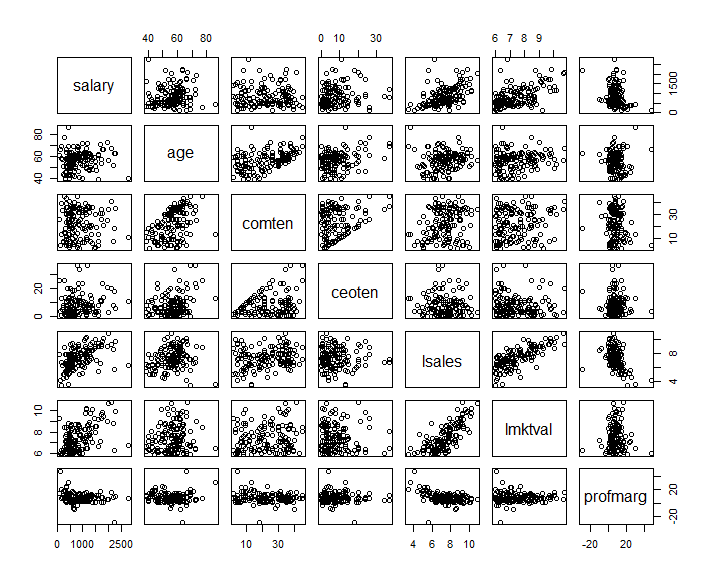
\includegraphics[width=.75\linewidth]{../Photo Of Result/B1_plotVriables.png}  
	\caption{Mối tương quan giữa các biến}
	\label{fig-b1:plot-vars}
\end{figure}
Tính độ tương quan giữa biến \texttt{salary} với 3 biến trên ta có:
\begin{figure}[H]
	\centering
	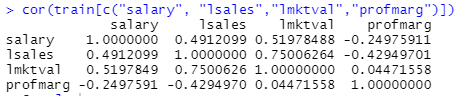
\includegraphics[width=.7\linewidth]{../Photo Of Result/B1_CorTable.PNG}  
	\caption{Mức độ tương quan giữa biến \texttt{lsales} và \texttt{promarg}}
	\label{fig-b1:corr-table}
\end{figure}

Xét bảng correlation giữa các biến độc lập với nhau và giữa các biến độc lập với biến phụ thuộc, ta thấy: Giữa hai biến \texttt{lmktval} và biến \texttt{lsales} có mối tương quan rất cao ($\approx 0.75$). Tuy nhiên biến \texttt{lmktval} lại có mối tương quan cao hơn với biến phụ thuộc \texttt{salary}. Mặt khác giữa biến \texttt{profmarg} và \texttt{lsales} cũng có mối tương quan cao ($\approx -0.42$). Nên ta loại bỏ biến \texttt{lsales} khỏi danh sách các biến được xét. (2)

Từ (1) và (2) ta có mô hình với đầy đủ các biến cần lựa chọn như sau:
\begin{equation}\label{eq-b1:full-model}
	\begin{split}
		\texttt{salary} 	= \beta_0 + &\beta_1 \times \texttt{age} + \beta_2 \times \texttt{college} + \beta_3 \times \texttt{grad} + \beta_4 \times \texttt{comten}\\
		+ &\beta_5\times \texttt{ceoten} + \beta_6\times \texttt{lmktval} + \beta_7\times \texttt{profmarg}
	\end{split}
\end{equation}


Thực hiện phân rã hai biến phân loại gồm \texttt{college} và \texttt{grad} trước khi thực hiện phương pháp  \textbf{Stepwise tiến} với \textbf{tiêu chuẩn AIC}.

Để đánh giá chất lượng mô hình ta chia tâp dữ liệu thành hai phần, training và testing, với tỷ lệ $8:2$ sau đó tiến hành phương pháp chọn biến trên tập training.

\subsection*{Chọn biến bằng phương pháp Stepwise tiến và tiêu chuẩn AIC}

\begin{figure}[H]
	\centering
	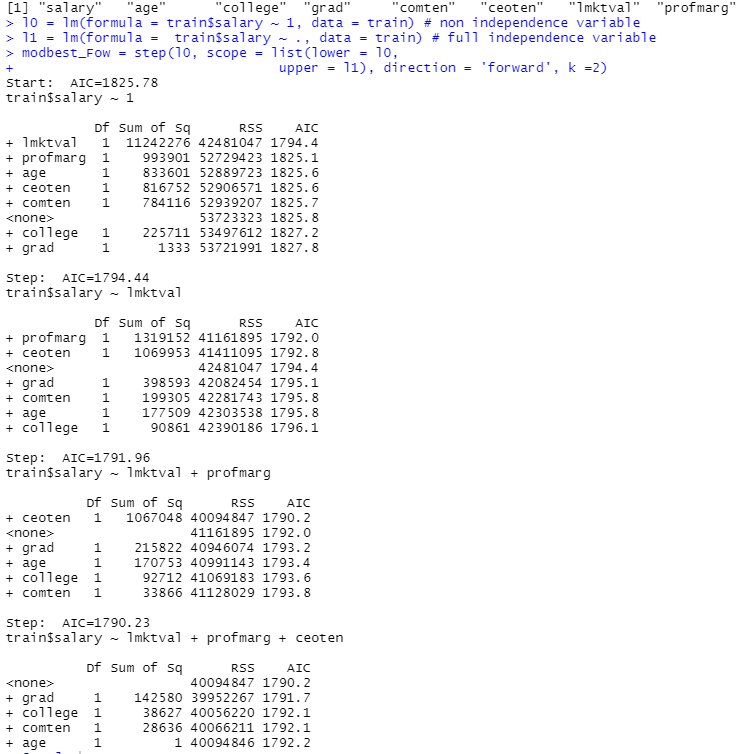
\includegraphics[width=\linewidth]{../Photo Of Result/B1_stepwiseForward.PNG}  
	\caption{Kết quả chọn biến theo phương pháp StepWise tiến với tiêu chuẩn AIC}
	\label{fig-b1:stepwise-forward}
\end{figure}

Tổng quan tiêu chuẩn AIC thì mô hình tốt là mô hình có giá trị AIC nhỏ nhất. Ở mô hình 1, biến \texttt{lmktval} được chọn vào mô hình vì có AIC nhỏ nhất trong tất cả các kết~hợp với các biến còn lại. Tương tự AIC được tính cho mô hình thêm biến thứ 2, \texttt{ceoten}, và biến thứ 3 là \texttt{ceoten} (hình \ref{ex1:model:1}).

\begin{figure}[H]
	\centering
	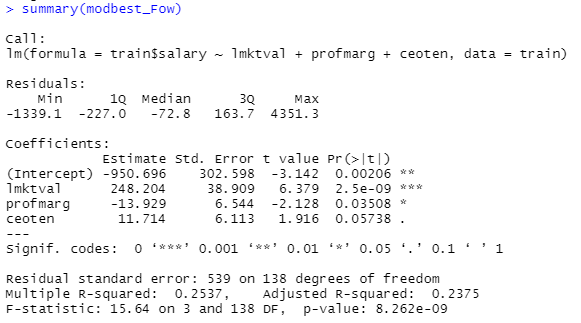
\includegraphics[width=.7\linewidth]{../Photo Of Result/B1_summary.PNG}  
	\caption{Kết quả hồi quy mô hình với các biến được chọn}
	\label{ex1:model:1}
\end{figure}

Với ba biến được chọn ở trên, mô hình \ref{eq-b1:full-model} trở thành mô hình mới:
\begin{equation}\label{1.2}
\texttt{salary} = -950.6 + 248.2 * \texttt{lmktval} - 13.9 *\texttt{profmarg} + 11.7  *\texttt{ceoten}
\end{equation}

Tuy nhiên ta nhận thấy biến \texttt{ceoten} có $\rho_{value} \ge \alpha$ (0.05738 $\ge$ 0.05) nên không có ý~nghĩa thống kê trong mô hình. Ta tiến hành bỏ biến \texttt{ceoten} và hồi quy mô hình với hai biến còn lại kết quả thu được từ phần mềm R như hình \ref{fig-b1:new-summary}:

\begin{figure}[H]
	\centering
	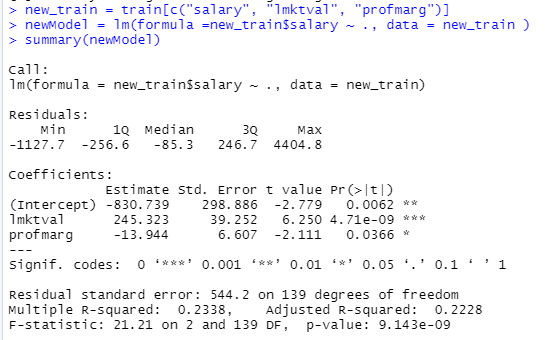
\includegraphics[width=.7\linewidth]{../Photo Of Result/B1_newsummary.PNG}  
	\caption{Kết quả hồi quy mô hình với hai biến còn lại}
	\label{fig-b1:new-summary}
\end{figure}

Mô hình thống kê mới:
\begin{equation}\label{1.3}
\texttt{salary} = -830.7 + 245.3 *\texttt{lmktval} -13.9 *\texttt{profmarg}
\end{equation}

Trường hợp này hai biến còn lại có ý nghĩa thống kê. Tuy nhiên mô hình được tạo bởi hai biến này chỉ giải thích được 23$\%$ sự biến thiên của biến phụ thuộc (hình \ref{fig-b1:new-summary}). Nguyên nhân dẫn tới kết quả thấp là do số lượng data ít, các biến giải thích ít không tạo nên mô hình đặc trưng được.

\subsection*{Kiểm tra trên tập test và nhận xét kết quả}

Thực hiện dự đoán trên tập dữ liệu test từ kết quả mô hình \ref{1.3} và dùng chỉ số đánh giá MSE (trung bình bình phương sai số) ta có:

\begin{figure}[H]
	\centering
	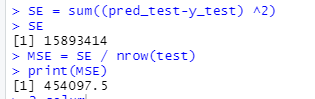
\includegraphics[width=.5\linewidth]{../Photo Of Result/B1_MSE.PNG}  
	\caption{Chỉ số đo lường kết quả MSE}
	\label{fig-b1:mse}
\end{figure}

Kết quả MSE $\approx$ 454097 lớn hơn nhiều so với giá trị trung bình $=887.5$ nên ta có thể thấy hai yếu tố gồm: giá thị trường (\texttt{lmktval}) và tỷ lệ phần trăm lợi nhuận (\texttt{profmarg}) là chưa đủ để giải thích mức độ tăng giảm của tiền lương của các giám đốc điều hành các tập~đoàn Hoa Kỳ. 

Để cải thiện kết quả mô hình ta nên tiến hành thu thập thêm dữ liệu và tiến hành lựa chọn biến dựa trên dữ liệu mới này. Bên cạnh đó có thể xem xét tới xem xét tới các nhân tố khác ảnh hưởng tới tiền lương của các giám đốc Hoa kỳ như: Lĩnh vực hoạt~động (ngân hàng, hàng không, công nghệ, vận tải...); mức lương trước đó; số năm kinh nghiệm, giới tính,...
	

